\documentclass{standalone}

\usepackage{amsmath,amsfonts,amssymb,amsthm,mathtools} 
\usepackage{fontspec}            % пакет для подгрузки шрифтов
\setmainfont{Impact}   % задаёт основной шрифт документа

% why do we need \newfontfamily:
% http://tex.stackexchange.com/questions/91507/
\newfontfamily{\cyrillicfonttt}{Impact}
\newfontfamily{\cyrillicfont}{Impact}
\newfontfamily{\cyrillicfontsf}{Impact}
% Иногда тех не видит структуры шрифтов. Эти трое бравых парней спасают ситуацию и доопределяют те куски, которые Тех не увидел.

\usepackage{unicode-math}     % пакет для установки математического шрифта
\setmathfont{Asana Math}      % шрифт для математики

\usepackage{polyglossia}      % Пакет, который позволяет подгружать русские буквы
\setdefaultlanguage{russian}  % Основной язык документа
\setotherlanguage{english}    % Второстепенный язык документа

\usepackage{pgf,tikz,pgfplots}
\usetikzlibrary{arrows,calc}
\usepackage{relsize} 

\usepackage{graphicx} 
\usepackage{rotating}
\usepackage{xcolor}
\usepackage{color}


\begin{document}

\begin{tikzpicture}[
        scale=2,
        dot/.style={circle,fill=black,minimum size=4pt,inner sep=0pt,
            outer sep=-1pt},
    ]
    
\begin{scope}[rotate=30]       
% Radius of regular polygons
  \newdimen\R
  \R=2cm
  \coordinate (center) at (0,0);
 \draw (0:\R)
     \foreach \x in {60,120,...,360} {  -- (\x:\R) }
              -- cycle (300:\R)
              -- cycle (240:\R)
              -- cycle (180:\R)
              -- cycle (120:\R)
              -- cycle (60:\R)
              -- cycle (0:\R)  [line width=1.9mm,color=black,fill=white,fill opacity=0];
\end{scope}
           
\node[text width=3.5cm] at (0.15,1.25) 
    {\Large Я НЕ ПОТНЫЙ,};
\node[inner sep=0pt] (russell) at (0,0)
    {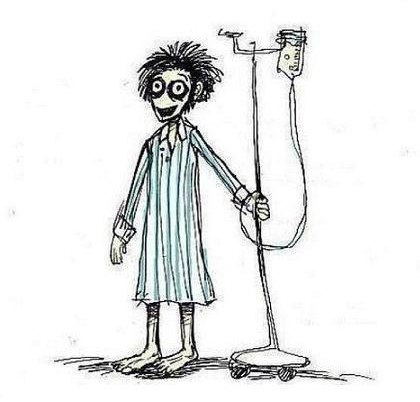
\includegraphics[scale=0.3]{pot.jpg}}; 
    \node[text width=3.5cm] at (0.28,-1.25) 
    {\Large Я ЖОСКИЙ!};
\end{tikzpicture}                       


\end{document}